\section{Generics Implementation in Programming Languages}\label{sec:java_generics}

There exist two common ways to implement generics in a programming language,
that are often described in literature as \emph{heterogeneous}
and \emph{homogeneous}~\cite{generics_categories}.
In the heterogeneous approach, the code is duplicated and specialized for each instance
of the generic parameters; this is the approach adopted by C++ \emph{templates}.
Conversely, the homogeneous approach is that provided by Java and .Net; in this case,
only one instance of the code is maintained and shared by all generic instances.
This implementation is based on the type \emph{erasure} mechanism, where the generic parameter
is replaced by the upwards bound of each instance, mostly often \<Object>.
Even though the heterogeneous approach is the safest, it is rarely applied, in particular
in resource-constrained applications, because the code size may dramatically increase
as a consequence of duplication~\cite{generics_embedded_systems}. For code in blockchain,
the heterogeneous approach obliges one to reinstall all instantiations of the generic code,
with extra costs of gas, which makes it impractical.
Conversely, the homogeneous approach ensures a smaller consumption of resources.

\begin{figure*}[ht]
\centering
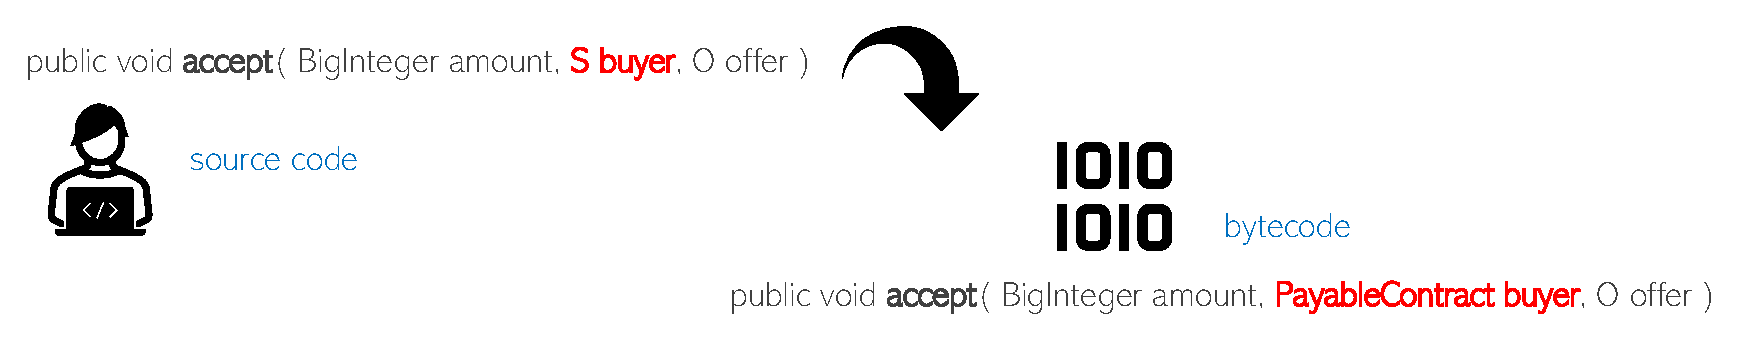
\includegraphics[width=0.8\linewidth]{figures/java_generics_erasure}
\caption{Example of generics implementation by erasure in Java.}
\label{figure.java_generics_erasure}
\end{figure*}

In order to understand the mechanism of erasure, consider for instance
the interface \<SharedEntity> in Fig.~\ref{fig:shared_entity} and its method \<accept>.
The functionality of \<SharedEntity> will be discussed later (Sec.~\ref{sec:shared_entities}).
Here, it is relevant to consider only how its generic type parameters get compiled.
Namely, \<SharedEntity> uses two generic type parameters \<S> and \<O>, that must be provided
whenever a client creates a concrete implementation of the interface.
Such generic parameters have an upper bound: \<S> can only be a subtype of \<PayableContract>,
while \<O> can only be a subtype of {\codesize\texttt{Offer<S>}}. If one checks the bytecode
generated for \<SharedEntity>, she will see that \<accept> is declared, in bytecode, as
\<void accept(BigInteger amount, PayableContract buyer, Offer offer)>, that is,
the two type variables \<S> and \<O> have been \emph{erased} and replaced with their
respective upper bound, as illustrated in Fig.\,\ref{figure.java_generics_erasure}.



Erasure weakens the type information of the compiled code. It is the responsibility of the
compiler to guarantee that types are still respected, in all implementations of \<SharedEntity>.
In Java, the compiler guarantees type correctness and the Java language remains strongly-typed,
also in the presence of generic types,
if no \emph{unchecked operations} are performed~\cite{NaftalinW06} (such as casts to generic types,
that are unchecked for a limitation of the Java bytecode).
However, this guarantee applies to Java source code compiled by the Java compiler,
not to bytecode that can be generated manually, in order to attack instances of
the \<SharedEntity> class, as shown later.
